\section{An efficient Parallel \texorpdfstring{\epsolute{}}{Epsolute}}\label{section:range-persistent:prallel-dp-oram}

	While the previously described scheme is a secure and correct \acrshort{cdpodb}, a single-threaded implementation may be prohibitively slow in practice.
	To bring the performance closer to real-world requirements, we need to be able to scale the algorithm horizontally.
	In this section, we describe an upgrade of \epsolute{} --- a scalable parallel solution.

	We suggest two variants of parallel \epsolute{} protocol.
	Both of them work by operating \oramsNumber{} \acrshortpl{oram} and randomly assigning to each of them $\nicefrac{n}{\oramsNumber}$ database records.
	For each query, we utilize the index \indexI{} to find the required records from the corresponding \acrshortpl{oram}.
	For each \acrshort{oram}, we execute a separate thread to retrieve the records.
	The threads work in parallel and there is no need for locking, since each \acrshort{oram} works independently from the rest.
	We present two methods that differ in the way they build and store \acrshort{dp} structure \serverDS{}, and hence the number of \acrshort{oram} requests they make.

	\subsection{\texorpdfstring{No-$\gamma$-method}{No-gamma-method}: \acrshort{dp} structure per \acrshort{oram}}

		In \protocolNoGamma{}, for each \acrshort{oram} / subset of the dataset, we build a \acrshort{dp} index the same way as described in \cref{section:range-persistent:dp-oram}.
		We note that \cref{theorem:composition} for disjoint datasets applies to this construction: the privacy budget $\epsilon$ for the construction is the largest (least private) among the $\epsilon$'s of the \acrshort{dp} indices for each \acrshort{oram} / subset of the dataset.

		The communication efficiency changes because
		\begin{enumerate*}[label={(\roman*)}]
			\item
				we essentially add \oramsNumber{} record subsets in order to answer a query, each having at most $\alpha$ extra random records, and
			\item
				each \acrshort{oram} holds fewer records than before, resulting in a tree of height $\log \frac{\dataSize}{\oramsNumber}$.
		\end{enumerate*}

		However, we cannot expect that the records required for each query are equally distributed among the different \acrshortpl{oram} in order to reduce the multiplicative communication cost from $\log \dataSize$ to $\frac{\log \dataSize}{\oramsNumber}$.
		Instead, we need to bound the worst case scenario which is represented by the maximum number of records from any \acrshort{oram} that is required to answer a query.
		This can be computed as follows.

		Let $X_j$ be $1$ if a record for answering query \query{} is in a specific $\algo{ORAM}_j$, and $0$ otherwise.
		Due to the random assignment of records to \acrshortpl{oram}, $\probability{X_j = 1} = \nicefrac{1}{\oramsNumber}$.
		Assume that we need $k_0$ records in order to answer query \query{}.
		The maximum number of records from $\algo{ORAM}_j$ in order to answer \query{} is bounded as follows.

		\begin{equation}\label{equation:gamma}
			\probability{ \sum_{i=1}^{k_0} X_i > ( 1 + \gamma ) \frac{k_0}{\oramsNumber} } \leq \exp{ \left( - \frac{ k_0 \gamma^2 }{ 3 \oramsNumber } \right) }
		\end{equation}

		Finally, we need to determine the value of $\gamma$ such that $\exp{ \left( - \frac{ k_0 \gamma^2 }{ 3 \oramsNumber } \right) }$ is smaller than the value $\beta$.
		Thus, $\gamma = \sqrt{ \frac{-3 \oramsNumber \log \beta}{ k_0 } }$.
		The communication efficiency for each query type is described in the following corollary.

		\begin{corollary}\label{corollary:no-gamma}
			Let \protocolNoGamma{} be an outsourced database system with storage efficiency \efficiency{1}{0}.
			Depending on the query type, \protocolNoGamma{} offers the following communication efficiency.
			\begin{description}
				\item[Range queries] $\efficiency{\left( 1 + \sqrt{ \frac{- 3 \oramsNumber \log \beta}{k_0} } \right) \log \frac{\dataSize}{\oramsNumber} }{ \frac{ \log^{1.5} \domainSize}{ \epsilon } \oramsNumber \log \dataSize }$
				\item[Point queries] $\efficiency{\left( 1 + \sqrt{ \frac{- 3 \oramsNumber \log \beta}{k_0} } \right) \log \frac{\dataSize}{\oramsNumber} }{ \frac{ \log \domainSize}{ \epsilon } \oramsNumber \log \dataSize }$
			\end{description}

			Then, \protocolNoGamma{} satisfies $\epsilon$-differential privacy for some $\epsilon$.
		\end{corollary}

		In our experiments, we set \oramsNumber{} as a constant depending on the infrastructure.
		However, if \oramsNumber{} is set as $\bigO{\log n}$, the total communication overhead of the construction will still exceed the lower-bound presented in \cite{multi-server-orams}.

	\subsection{\texorpdfstring{$\gamma$-method}{Gamma-method}: shared \acrshort{dp} structure}\label{section:range-persistent:prallel-dp-oram:gamma}

		In \protocolGamma{}, we maintain a single shared \acrshort{dp} structure \serverDS{}.
		When a query is issued, we must ensure that the number of records retrieved from every \acrshort{oram} is the same.
		As such, depending on the required noisy number of records $\tilde{k}_0$, we need to retrieve at most $( 1 + \gamma ) \frac{ \tilde{k}_0 }{\oramsNumber}$ records from each \acrshort{oram}, see \cref{equation:gamma}, for $\gamma = \sqrt{ \frac{-3 \oramsNumber \log \beta}{ \tilde{k}_0 } }$.
		Setting $\tilde{k}_0 = k_0 + \frac{\log^{1.5} \domainSize}{\epsilon}$ for range queries and $\tilde{k}_0 = k_0 + \frac{\log \domainSize}{\epsilon}$ for point queries, the communication efficiency is as follows.

		\begin{corollary}\label{corollary:gamma}
			Let \protocolGamma{} be an outsourced database system with storage efficiency \efficiency{1}{0}.
			Depending on the query type, \protocolGamma{} offers the following communication efficiency.
			\begin{description}
				\item[Range queries] $\efficiency{ \left( 1 + \sqrt{ \frac{-3 \oramsNumber \log \beta}{k_0 + \frac{ \log^{1.5} \domainSize }{ \epsilon }} }\right) \log \frac{\dataSize}{\oramsNumber} \left( 1 + \frac{\log^{1.5} \domainSize}{\epsilon} \right) }{0}$
				\item[Point queries] $\efficiency{ \left( 1 + \sqrt{ \frac{-3 \oramsNumber \log \beta}{k_0 + \frac{ \log \domainSize }{ \epsilon }} }\right) \log \frac{\dataSize}{\oramsNumber} \left( 1 + \frac{\log \domainSize}{\epsilon} \right) }{0}$
			\end{description}
			Then, \protocolGamma{} satisfies $\epsilon$-differential privacy for some $\epsilon$.
		\end{corollary}

		\protocolGamma{} is depicted in \cref{algorithm:dp-oram-parallel}.
		There are a few extensions to the subroutines and notation from \cref{algorithm:dp-oram}.
		\algo{CreateIndex} and \algo{Lookup} now build and query the index which maps a search key to a pair --- the record ID and the \acrshort{oram} ID (1 to \oramsNumber{}) which stores the record.
		\Crefrange{algorithm:dp-oram-parallel:gamma:setup:line-4}{algorithm:dp-oram-parallel:gamma:setup:line-6} of \cref{algorithm:dp-oram-parallel} \protocolSetup{} repeat for each \acrshort{oram} and operate on the records partitioned for the given \acrshort{oram} using hash function \algo{H} on the record ID\@.
		A shared \acrshort{dp} structure is created with the sanitizer \algo{A} (\cref{algorithm:dp-oram-parallel:gamma:setup:line-7}).
		In \cref{algorithm:dp-oram-parallel} \protocolQuery{}, the total number of \acrshort{oram} requests is computed once (\cref{algorithm:dp-oram-parallel:gamma:query:line-4}).
		\Crefrange{algorithm:dp-oram-parallel:gamma:query:line-5}{algorithm:dp-oram-parallel:gamma:query:line-7} repeat for each \acrshort{oram} and operate on the subset of records stored in the given \acrshort{oram}.
		Note that \user{} and \server{} implicitly maintain \oramsNumber{} \acrshort{oram} states, and the algorithm uses the $(\algo{A}, \algo{B})$ sanitizer defined in \cref{section:range-persistent:dp-oram}.

		Note that we guarantee privacy and access pattern protection on a record level.
		Each \acrshort{oram} gets accessed at least once (much more than once for a typical query) thus the existence of a particular result record in a particular \acrshort{oram} is hidden.

	\subsection{Practical improvements}\label{section:range-persistent:dp-improvements}

		Here we describe the optimizations aimed at bringing the construction's performance to the real-world demands.

		\subsubsection{\acrshort{oram} request batching}\label{section:range-persistent:dp-improvements:oram-batching}

			We have noticed that although the entire set of \acrshort{oram} requests for each query is known in advance, the requests are still executed sequentially.
			To address this inefficiency, we have designed a way to combine the requests in a batch and reduce the number of network requests to the bare minimum.
			We have implemented this method over PathORAM, which we use for the $(\eta_1, \eta_2)$-\acrshort{oram} protocol, but the idea applies to most tree-based \acrshortpl{oram} (similar to \cite{parallel-oram-improved}).

			Our optimization utilizes the fact that all PathORAM leaf IDs are known in advance and paths in a tree-based storage share the buckets close to the root.
			The core idea is to read all paths first, processes the requests and and then write all paths back.
			This way the client makes a single \texttt{read} request, which is executed much faster than many small requests.
			Requests are then processed in main memory, including re-encryptions.
			Finally, the client executes the \texttt{write} requests using remapped leaves as a single operation, saving again compared to sequential execution.

			This optimization provides up to \textbf{8 times} performance boost in our experiments.
			We note that the gains in speed and \acrshort{io} overhead are achieved at the expense of main memory, which is not an issue given that the memory is released after a batch, and our experiments confirm that.
			The security guarantees of PathORAM are maintained with this optimization, since the security proof in \cite[Section 3.6]{path-oram} still holds. % chktex 2
			Randomized encryption, statistically independent remapping of leaves, and stash processing do not change.

		\subsubsection{Lightweight \acrshort{oram} servers}\label{section:range-persistent:dp-improvements:three-tier}

			We have found in our experiments that na\"{\i}ve increase of the number of \acrshort{cpu} cores and gigabytes of memory does not translate into linear performance improvement after some threshold.
			Investigating the observation we have found that the \epsolute{} protocol, executing parallel \acrshort{oram} protocols, is highly intensive with respect to main memory access, cryptographic operations and network usage.
			The bottleneck is the hardware --- we have confirmed that on a single machine the memory and network are saturated quickly preventing the linear scaling.

			\begin{figure}[ht!]
	\centering
	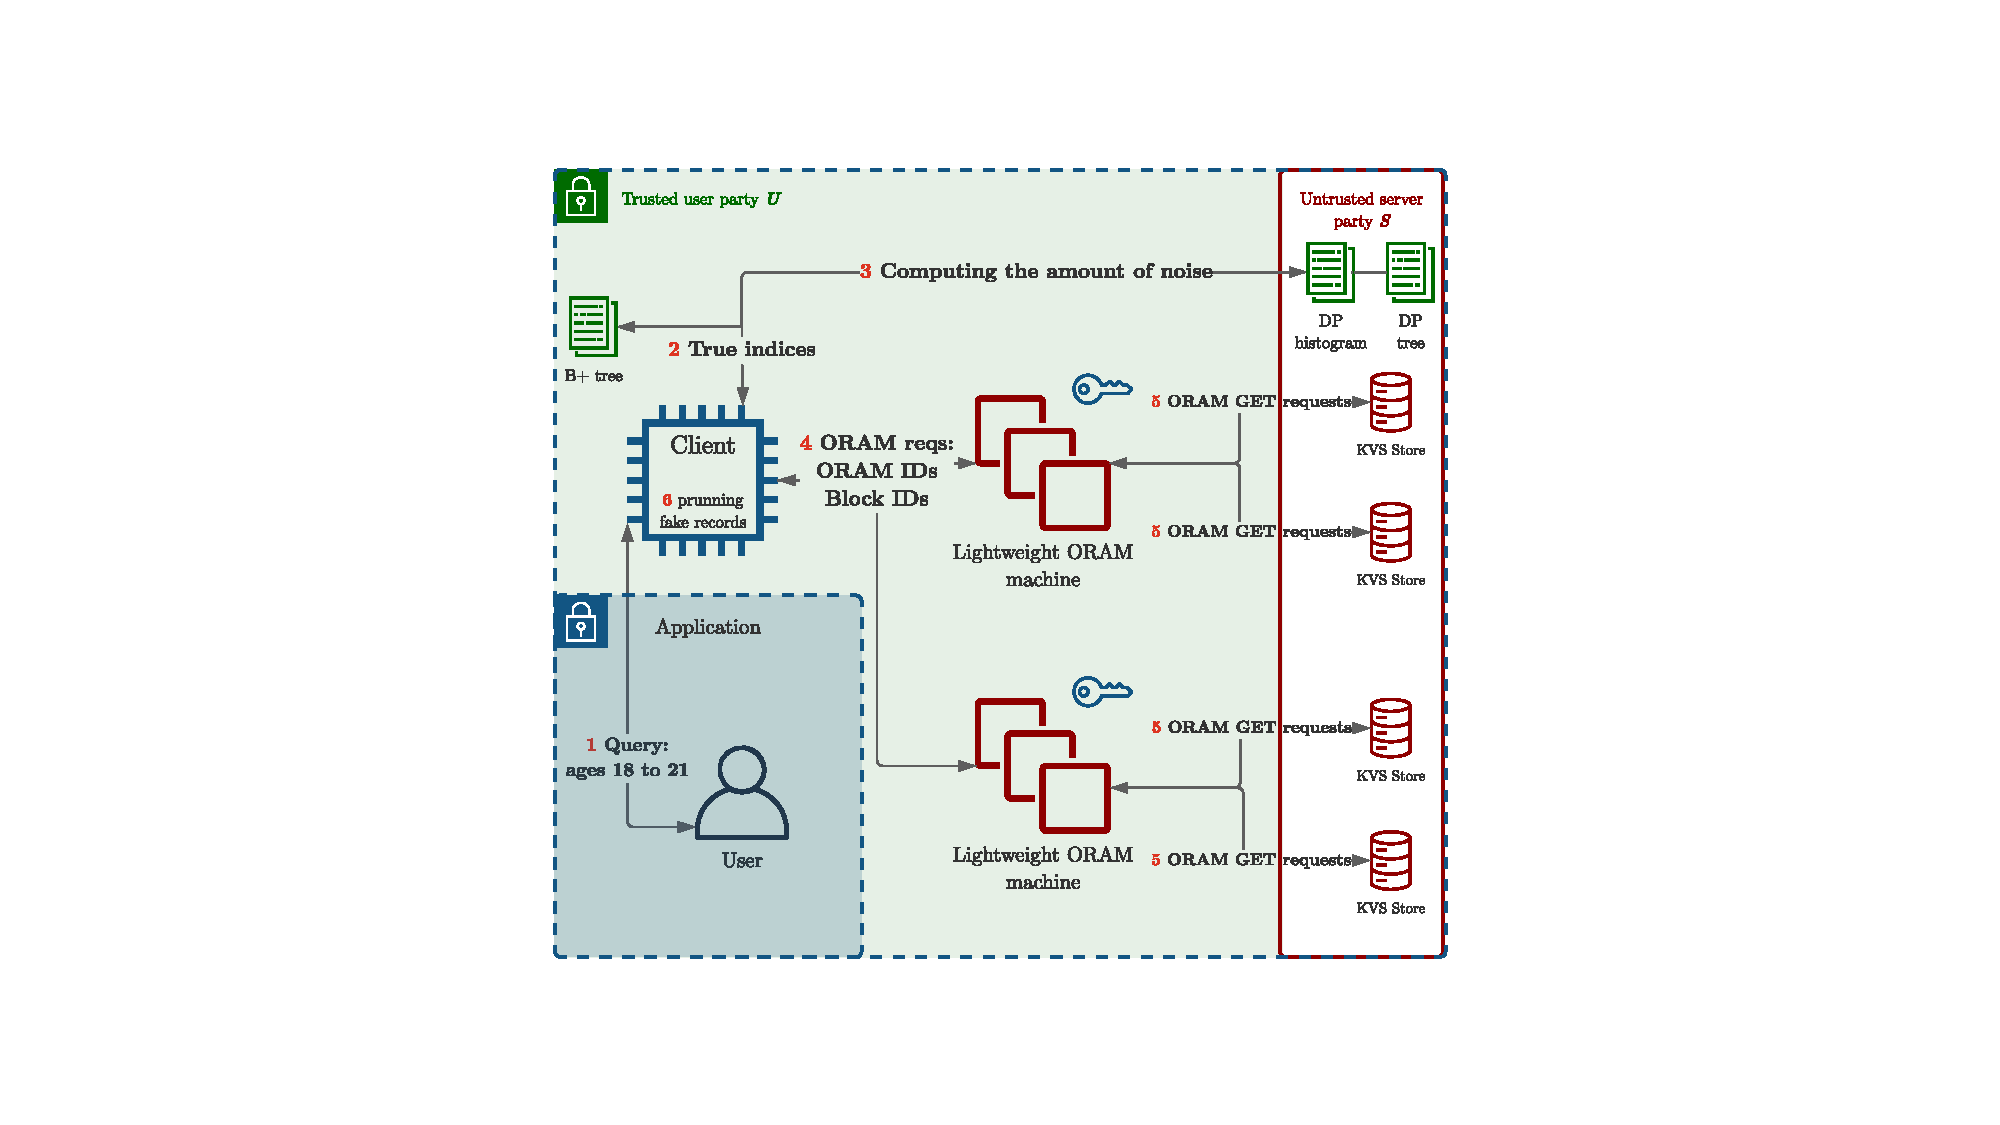
\includegraphics[width=\linewidth]{three-layers}
	\caption[Lightweight \acrshort{oram} machines diagram]{
		Lightweight \acrshort{oram} machines diagram.
		A \emph{user} sends a query to \user{} modeled as the \emph{client} machine, which uses local \emph{data index} and \emph{\acrshort{dp} structures} to prepare a set of \acrshort{oram} requests, which are sent to respective \emph{\acrshort{oram} machines}.
		These machines execute the \acrshort{oram} protocol against the \emph{untrusted storage} of \server{}.
	}%
	\label{figure:three-tier}
\end{figure}


			To address the problem, we split the user party \user{} into multiple lightweight machines that are connected locally to each other and reside in a single trust domain (e.g., same data center).
			Specifically, we maintain a \emph{client machine} that receives user requests and prepares \acrshort{oram} \texttt{read} requests, and up to \oramsNumber{} lightweight \emph{\acrshort{oram} machines}, whose only job is to run the \acrshort{oram} protocols in parallel.
			See \cref{figure:three-tier} for the schematic representation of the architecture.
			We emphasize that \user{} is still a single party, therefore, the security and correctness guarantees remain valid.

			The benefit of this approach is that each of the lightweight machines has its own hardware stack.
			Communication overhead among \user{} machines is negligible compared to the one between \user{} and \server{}.
			The approach is also flexible: it is possible to use up to \oramsNumber{} \acrshort{oram} machines and the machines do not have to be identical.
			Our experiments show that when the same number of \acrshort{cpu} cores and amount of memory are consumed the efficiency gain is up to \textbf{5 times}.
